\section{Experimental Study}
\label{sec:exp}
In this section, we evaluate the efficiency and scalability of our proposed parallel GCMP detectors on real trajectory datasets. All the experiments are carried out in a cluster with $12$ nodes, each equipped with four quad-core $2.2$GHz Intel processors, $32$GB memory and gigabit Ethernet. 

\textbf{Environment Setup}: We use Yarn\footnote{\url{http://hadoop.apache.org/docs/current/hadoop-yarn/hadoop-yarn-site/YARN.html}} to manage our cluster. We pick one machine as Yarn's master node, and for each of the remaining machines, we reserve one core and $2$GB memory for Yarn processes. We deploy our GCMP detector on Apache Spark 1.5.2~\cite{zaharia2012resilient} with the remaining $11$ nodes as the computing nodes.
To fully utilize the computing resources, we configure each node to run five executors, each taking three cores and $5$GB memory. In Spark, one of the $55$ executors is taken as the Application Master for coordination, therefore our setting results in $54$ executors. \revised{We set the number of partitions to be $486$ to fully utilize the parallelism provided by the multi-threading of every core.}
All our implementations as well as cluster setups are open-sourced in Github\footnote{\url{https://github.com/fanqi1909/TrajectoryMining/}}.

\textbf{Datasets}: We use three real trajectory datasets in different application scenarios:
\begin{itemize}
\item{Shopping}\footnote{\url{http://www.irc.atr.jp/crest2010_HRI/ATC_dataset/}}: The dataset contains
  trajectories of visitors in the ATC shopping center in Osaka. To better capture the indoor activities, the visitor locations are sampled every half second, resulting in $13,183$ long trajectories. 
\item{GeoLife}~\footnote{\url{http://research.microsoft.com/en-us/projects/geolife/}}: The dataset essentially keeps all the travel records of 182 users for a period
of over three years, including multiple kinds of transportation modes (walking, driving and taking public
transportation). For each user, the GPS information is collected periodically and 91 percent of the trajectories
are sampled every 1 to 5 seconds.
\item{Taxi}~\footnote{Taxi is our proprietary dataset}: The dataset tracks the trajectories of $15,054$ taxies in Singapore. For each taxi, the GPS information are continually collected for one entire month with the sampling rate around 30 seconds.
\end{itemize}


\textbf{Preprocessing}: We replace timestamps with global sequences (starting from $1$) for each dataset. 
We set a fixed sampling rate for each dataset (i.e., GeoLife = 5 seconds, Shopping=0.5 seconds, Taxi = 30 seconds)
and use linear interpolation to fill missing values.
%For each dataset, we set a fixed sampling rate (CLEARLY STATE THE SAMPLING RATE FOR EACH DATASET) and use linear interpolation to fill missing values. 
%Finally, we obtain a set of trajectories with equal length. 
%Finally, we obtain a set of dense trajectories with equal length. 
For the clustering method, we use DBSCAN~\cite{ester1996density} and customize its two parameters $\epsilon$ (proximity threshold) and $minPt$ (the minimum number of points required to form a dense region). We set $\epsilon=5$, $minPt=10$ for GeoLife and Shopping datasets; and $\epsilon=20$, $minPt=10$ for Taxi dataset. Note that other clustering methods or settings can also be applied. 
%The clustered snapshots are stored in HDFS as $\langle t, S_t \rangle$ pair, where $t$ is the timestamp, $S_t$ contains the clusters at snapshot $t$. 
After preprocessing, the statistics of the three datasets are listed in Table~\ref{exp:dataset}. 

\begin{table} [h]
\center
\small
\begin{tabular}{|l|l|l|l|}
\hline
 \textbf{Attributes}& \textbf{Shopping} &  \textbf{GeoLife} &  \textbf{SingTaxi} \\ 
\hline 
\# objects  & 13,183 & 18,670 & 15,054\\ 
\hline
%\# average ts & 3,114  & 2,924 & 19,667 \\ 
%\hline
\# data points  & 41,052,242 & 54,594,696 & 296,075,837\\ 
\hline
\# snapshots  & 16,931 & 10,699 & 44,364\\ 
\hline
\# clusters  & 211,403  & 206,704& 536,804\\
\hline
avg. cluster size  & 171 & 223 & 484\\
\hline
\end{tabular}
\caption{Statistics of datasets.}
\label{exp:dataset}
\end{table}

\textbf{Parameters}: To systematically study the performance of
our algorithms, we conduct experiments on various parameter settings. The parameters to be evaluated are listed in Table~\ref{tbl:parameters}, with default settings in bold. 
\begin{table}[h]
\small
\begin{tabular}{c|l|l}
\hline 
\textbf{Variables} & \textbf{Meaning} & \textbf{Values} \\ 
\hline 
M & min size of object set &  5, 10,  \textbf{15}, 20, 25 \\ 
\hline 
K & min duration & 120, 150, \textbf{180}, 210, 240 \\ 
\hline 
L & min local duration & 10, 20, \textbf{30}, 40,50 \\ 
\hline 
G & max gap & 10, 15, \textbf{20}, 25, 30 \\ 
\hline
$O_r$ & ratio of objects & 20\%,40\%, 60\%, 80\%, \textbf{100\%} \\ \hline
$T_r$ & ratio of snapshots & 20\%,40\%, 60\%, 80\%, \textbf{100\%} \\ \hline
N & number of machines & 1, 3, 5, 7, 9, \textbf{11}\\ 
\hline 
\end{tabular} 
\caption{Variables and their default values.}
\label{tbl:parameters}
\end{table}

\subsection{Performance Evaluation}
\begin{figure*}[t]
\centering
    \begin{subfigure}[b]{0.16\textwidth}
        \includegraphics[width=\textwidth]{/exp/performance/shopping_vary_M.eps}
        \caption{Shopping vary $M$}
    \end{subfigure}
    \begin{subfigure}[b]{0.16\textwidth}
        \includegraphics[width=\textwidth]{/exp/performance/shopping_vary_K.eps}
        \caption{Shopping vary $K$}
    \end{subfigure}
    \begin{subfigure}[b]{0.16\textwidth}
        \includegraphics[width=\textwidth]{/exp/performance/shopping_vary_L.eps}
        \caption{Shopping vary $L$}
    \end{subfigure}
       \begin{subfigure}[b]{0.16\textwidth}
        \includegraphics[width=\textwidth]{/exp/performance/shopping_vary_G.eps}
        \caption{Shopping vary $G$}
    \end{subfigure}
	\begin{subfigure}[b]{0.16\textwidth}
	 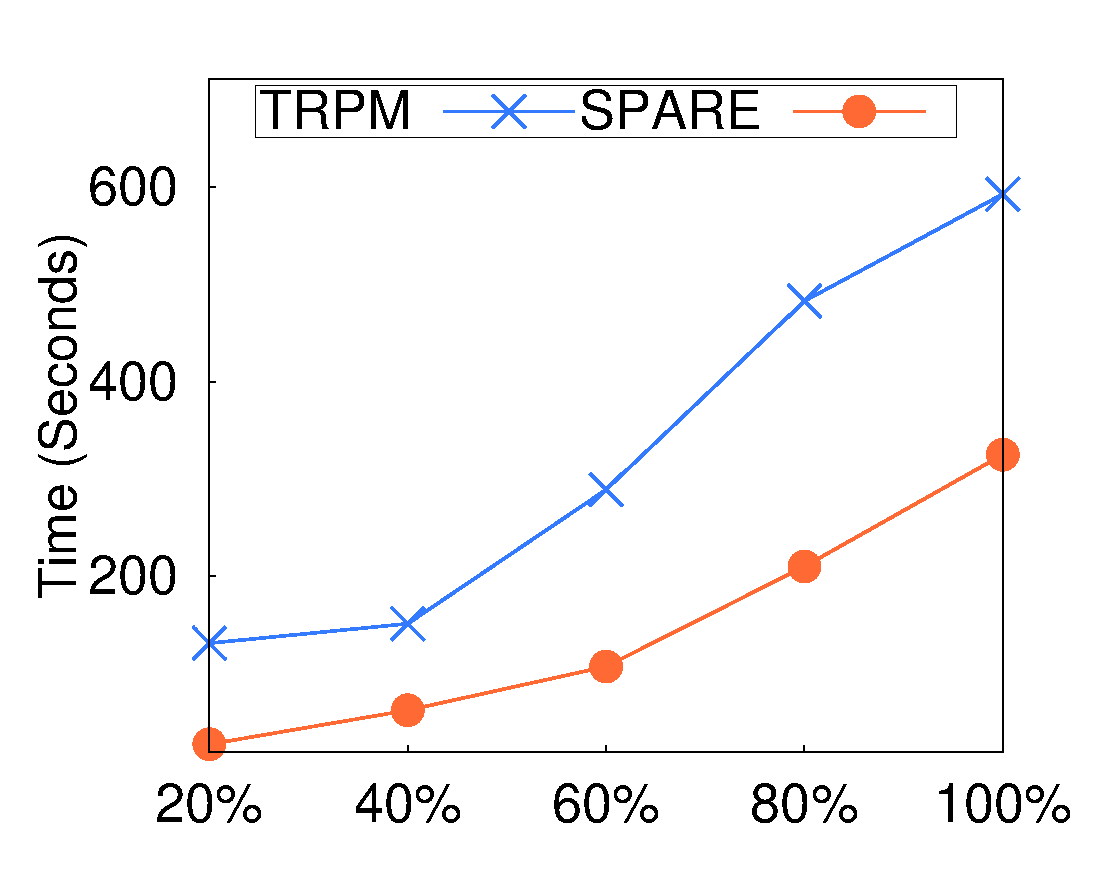
\includegraphics[width=\textwidth]{/exp/performance/shopping_vary_o.eps}
        \caption{Shopping vary $O_r$}
    \end{subfigure}
        \begin{subfigure}[b]{0.16\textwidth}
	 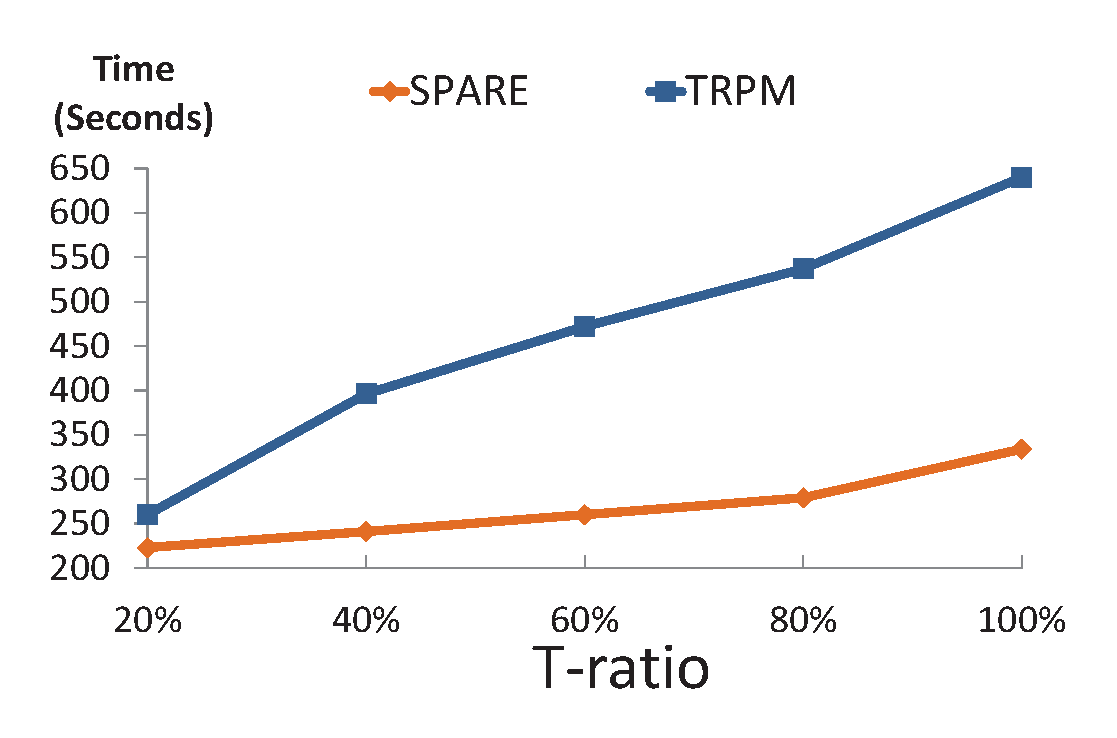
\includegraphics[width=\textwidth]{/exp/performance/shopping_vary_t.eps}
        \caption{Shopping vary $T_r$}
    \end{subfigure}
        
	\begin{subfigure}[b]{0.16\textwidth}
        \includegraphics[width=\textwidth]{/exp/performance/geolife_vary_M.eps}
        \caption{GeoLife vary $M$}
    \end{subfigure}
    \begin{subfigure}[b]{0.16\textwidth}
        \includegraphics[width=\textwidth]{/exp/performance/geolife_vary_K.eps}
        \caption{GeoLife vary $K$}
    \end{subfigure}
    \begin{subfigure}[b]{0.16\textwidth}
        \includegraphics[width=\textwidth]{/exp/performance/geolife_vary_L.eps}
        \caption{GeoLife vary $L$}
    \end{subfigure}
       \begin{subfigure}[b]{0.16\textwidth}
        \includegraphics[width=\textwidth]{/exp/performance/geolife_vary_G.eps}
        \caption{GeoLife vary $G$}
    \end{subfigure}       
 	 \begin{subfigure}[b]{0.16\textwidth}
        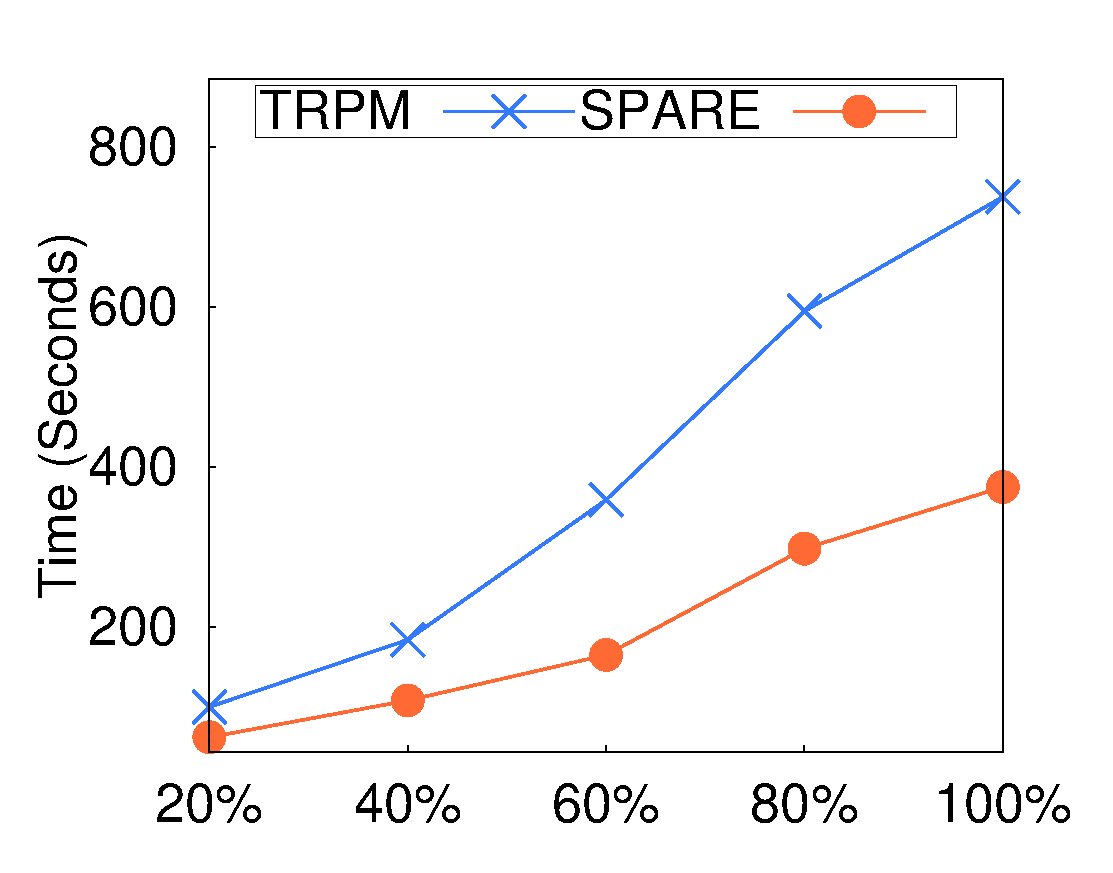
\includegraphics[width=\textwidth]{/exp/performance/geolife_vary_o.eps}
        \caption{GeoLife vary $O_r$}
    \end{subfigure}
 	\begin{subfigure}[b]{0.16\textwidth}
        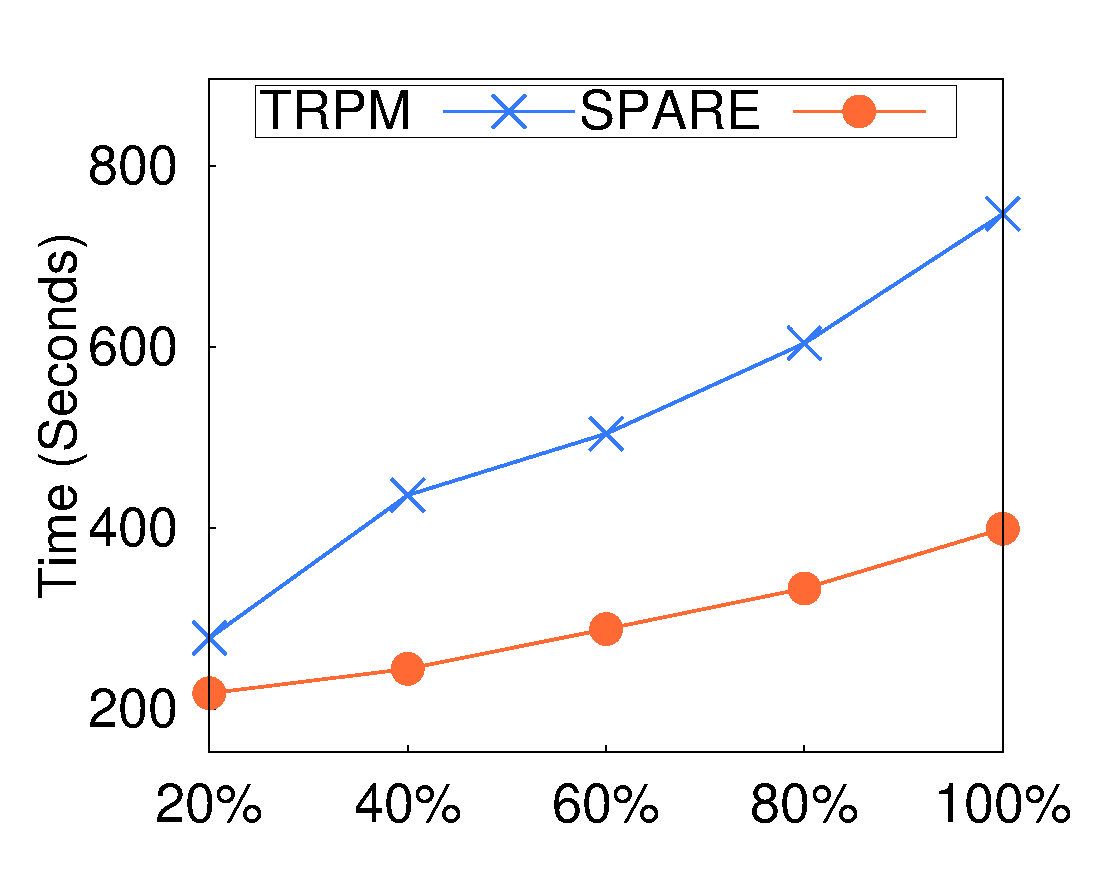
\includegraphics[width=\textwidth]{/exp/performance/geolife_vary_t.eps}
        \caption{GeoLife vary $T_r$}
    \end{subfigure}    
    
    \begin{subfigure}[b]{0.16\textwidth}
        \includegraphics[width=\textwidth]{/exp/performance/taxi_vary_M.eps}
        \caption{Taxi vary $M$}
    \end{subfigure}
    \begin{subfigure}[b]{0.16\textwidth}
        \includegraphics[width=\textwidth]{/exp/performance/taxi_vary_K.eps}
        \caption{Taxi vary $K$}
    \end{subfigure}
    \begin{subfigure}[b]{0.16\textwidth}
        \includegraphics[width=\textwidth]{/exp/performance/taxi_vary_L.eps}
        \caption{Taxi vary $L$}
    \end{subfigure}
       \begin{subfigure}[b]{0.16\textwidth}
        \includegraphics[width=\textwidth]{/exp/performance/taxi_vary_G.eps}
        \caption{Taxi vary $G$}
    \end{subfigure}   
	 \begin{subfigure}[b]{0.16\textwidth}
        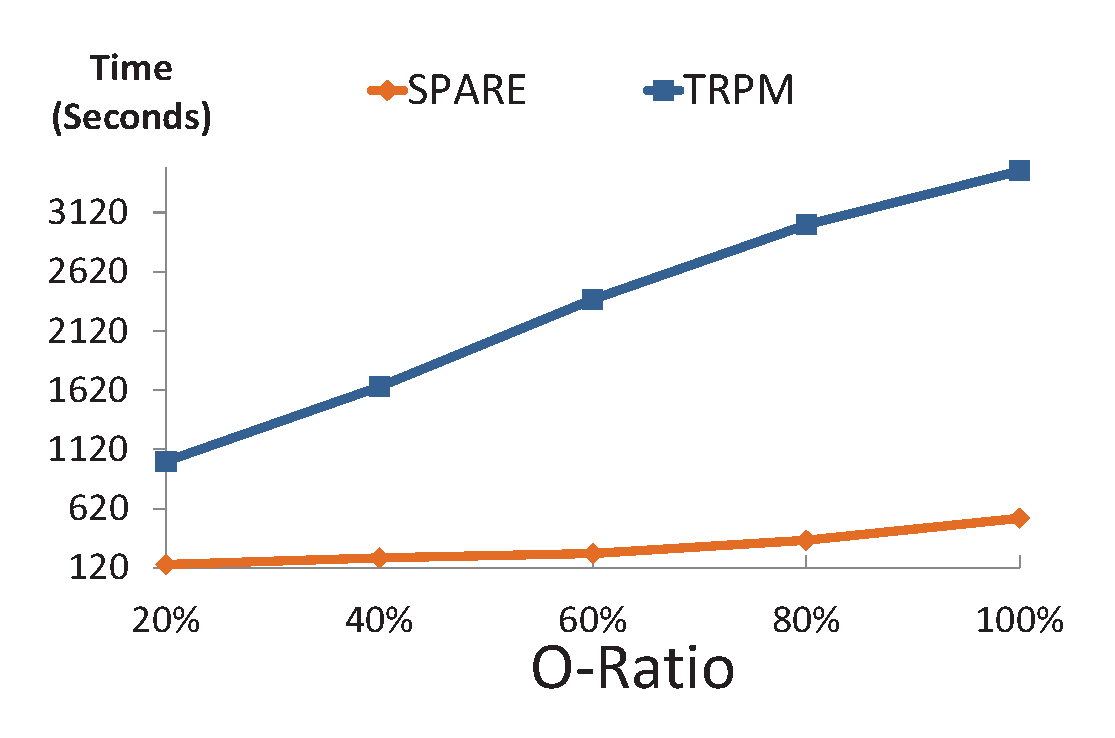
\includegraphics[width=\textwidth]{/exp/performance/taxi_vary_o.eps}
        \caption{Taxi vary $O_r$}
    \end{subfigure}
    	 \begin{subfigure}[b]{0.16\textwidth}
        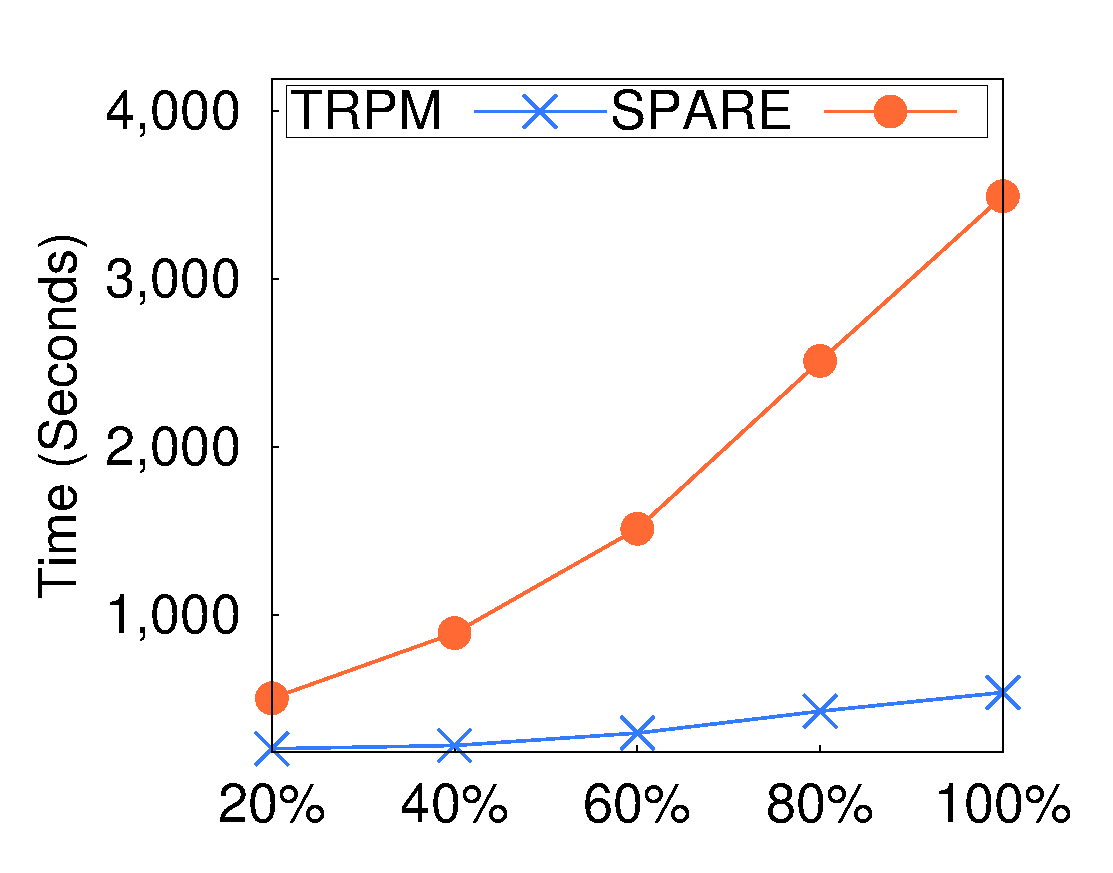
\includegraphics[width=\textwidth]{/exp/performance/taxi_vary_t.eps}
        \caption{Taxi vary $T_r$}
    \end{subfigure}      
        
\caption{Performance of SPARE and TRPM on real datasets under different pattern parameters.}
\label{exp:performance_vary}
\end{figure*}
\textbf{Varying $M$}: Figures~\ref{exp:performance_vary} (a),(g),(m)
present the performance with increasing $M$. The SPARE framework demonstrates a clear superiority over the TRPM framework, with 
a performance gain by a factor of  $2.7$ times in Shopping, $3.1$ times in GeoLife and
$7$ times in Taxi. As $M$ increases, the running time of both frameworks slightly improve because the number of clusters in each snapshot drops, generating fewer valid candidates.

\textbf{Varying $K$}: The performance with increasing $K$ is shown in Figure~\ref{exp:performance_vary} (b),(h),(n).  SPARE tends to run faster, whereas the performance of TRPM degrades dramatically. This is caused by the \emph{sequence simplification} procedure in SPARE, which can prune many candidates with large $K$. However, the line sweep algorithm in TRPM does not utilize such property for pruning. It takes longer time because more replicated data has to be handled in each partition.

\textbf{Varying $L$}: Figures~\ref{exp:performance_vary} (c),(i),(o) present the performances with increasing $L$. When $L=10$, SPARE can outperform TRPM by around $10$ times. We also observe that there is a significant performance improvement for TPRM when $L$ increases from $10$ to $20$ and later the running time drops smoothly. 
This is because $\eta$ is proportional to $O(K*G/L+L)$. When $L$ is small (i.e., from $10$ to $20$),
$\eta$ decreases drastically. As $L$ increases, $\eta$ varies less significantly.

\textbf{Varying $G$}: Figures~\ref{exp:performance_vary} (d),(j),(p) present the performances with increasing $G$.  TRPM is rather sensitive to $G$. When $G$ is relaxed to larger values, more valid patterns would be generated. TPRM has to set a higher replication factor and its running time degrades drastically when $G$ increases from $20$ to $30$. In contrast, with much more effective pruning strategy, our SPARE scales well with $G$. Particularly, SPARE is 14 times faster than TRPM when $G=20$ in GeoLife dataset.

\textbf{Varying $O_r$}: Figures~\ref{exp:performance_vary} (e),(k),(q) present the performances with increasing number of moving objects. Both TRPM and SPARE take longer time to find patterns in a larger database. We can see that the performance gap between SPARE and TRPM is widened as more objects are involved, which shows SPARE is more scalable.

\textbf{Varying $T_r$}: Figures~\ref{exp:performance_vary} (f),(l),(r) present 
the performances with increasing number of snapshots. As $T_r$ increases, SPARE scales much better than TRPM due to its effective pruning in the temporal dimension. 

\revised{
\textbf{Resources}: Table~\ref{tbl:resource} lists the system resources taken 
by TRPM and SPARE under the default setting. Both TRPM and SPARE are 
resource efficient as they only occupy less than 20\% 
of the available memory (i.e., 270GB) . Again, SPARE outperforms TRPM in both the execution time and the memory usage.

%The result also reveals the potential of the two solutions to handle larger trajectories. Again, SPARE outperforms TRPM in both execution time and memory usage which dues to the set of effective pruning procedures.

\begin{table}[h]
\small
\begin{tabular}{|l|c|c|c|c|}
\hline
\multicolumn{1}{|c|}{\textbf{Dataset}} & \textbf{Method} & \textbf{Time} & \textbf{Vcore-seconds} & \textbf{Memory} \\ \hline
\multirow{2}{*}{Shopping}              & TRPM            & 597                               & 90,859                 & 10,019               \\ %\cline{2-5} 
                                       & SPARE           & 237                               & 33,638                 & 8,613                \\ \hline
\multirow{2}{*}{Geolife}               & TRPM            & 747                               & 106,428                & 18,454               \\ %\cline{2-5} 
                                       & SPARE           & 341                               & 35,343                 & 14,369               \\ \hline
\multirow{2}{*}{Taxi}                  & TRPM            & 3,648                             & 503,460                & 51,691               \\ %\cline{2-5} 
                                       & SPARE           & 580                               & 68,580                & 35,912               \\ \hline
\end{tabular}
\caption{Resources taken for TRPM and SPARE. Time is in seconds representing observed performance. Vcore-seconds is the aggregate of time spent in each core. Memory is in MB representing the actual size of RDDs.}
\label{tbl:resource}
\end{table}
}
%\begin{figure}[h]
%\centering
%	\begin{subfigure}[b]{0.22\textwidth}
%	 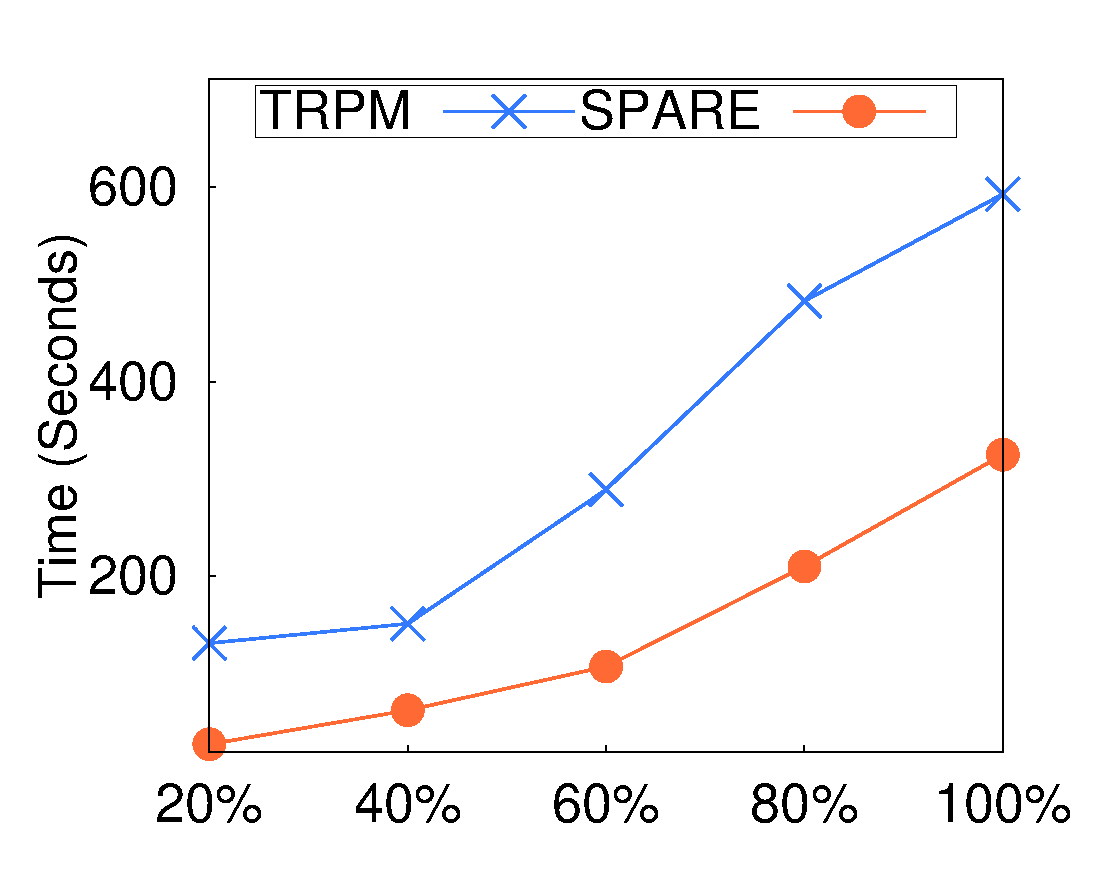
\includegraphics[width=\textwidth]{/exp/performance/shopping_vary_o.eps}
%        \caption{Shopping vary $O_r$}
%    \end{subfigure}
% 	 \begin{subfigure}[b]{0.22\textwidth}
%        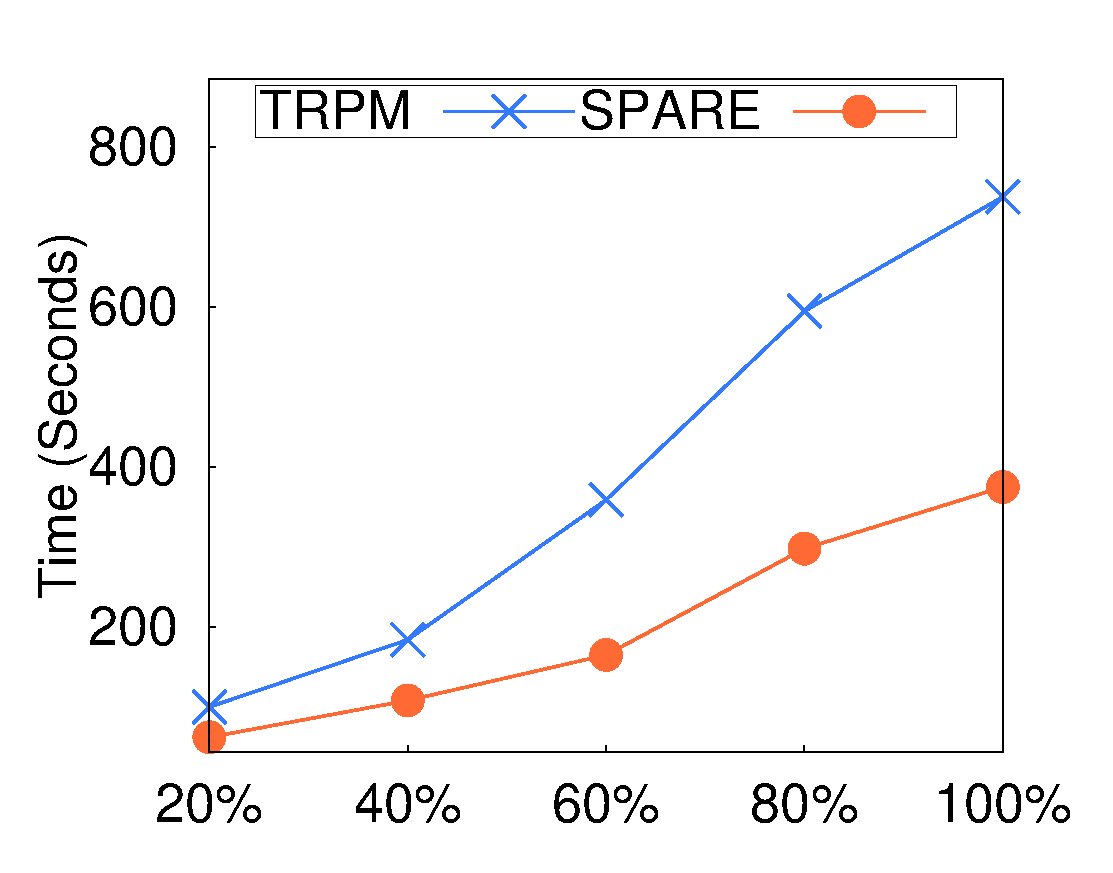
\includegraphics[width=\textwidth]{/exp/performance/geolife_vary_o.eps}
%        \caption{Geolife vary $O_r$}
%    \end{subfigure}
%    	 \begin{subfigure}[b]{0.22\textwidth}
%        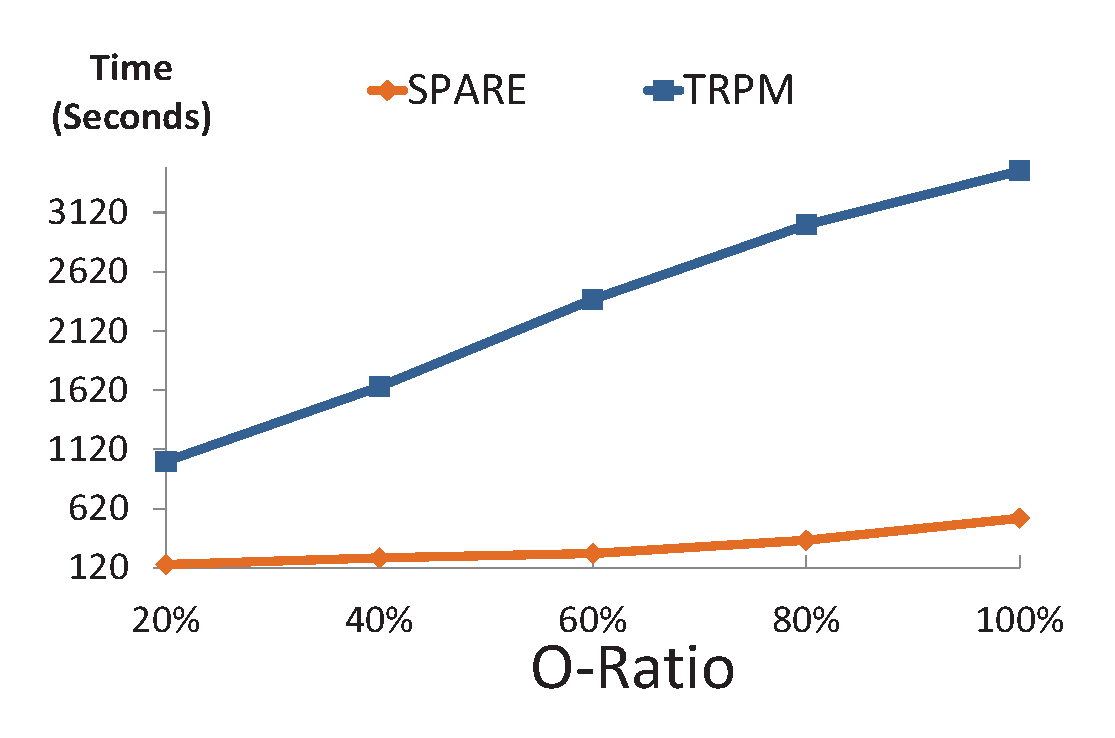
\includegraphics[width=\textwidth]{/exp/performance/taxi_vary_o.eps}
%        \caption{Taxi vary $O_r$}
%    \end{subfigure}
%    \begin{subfigure}[b]{0.22\textwidth}
%	 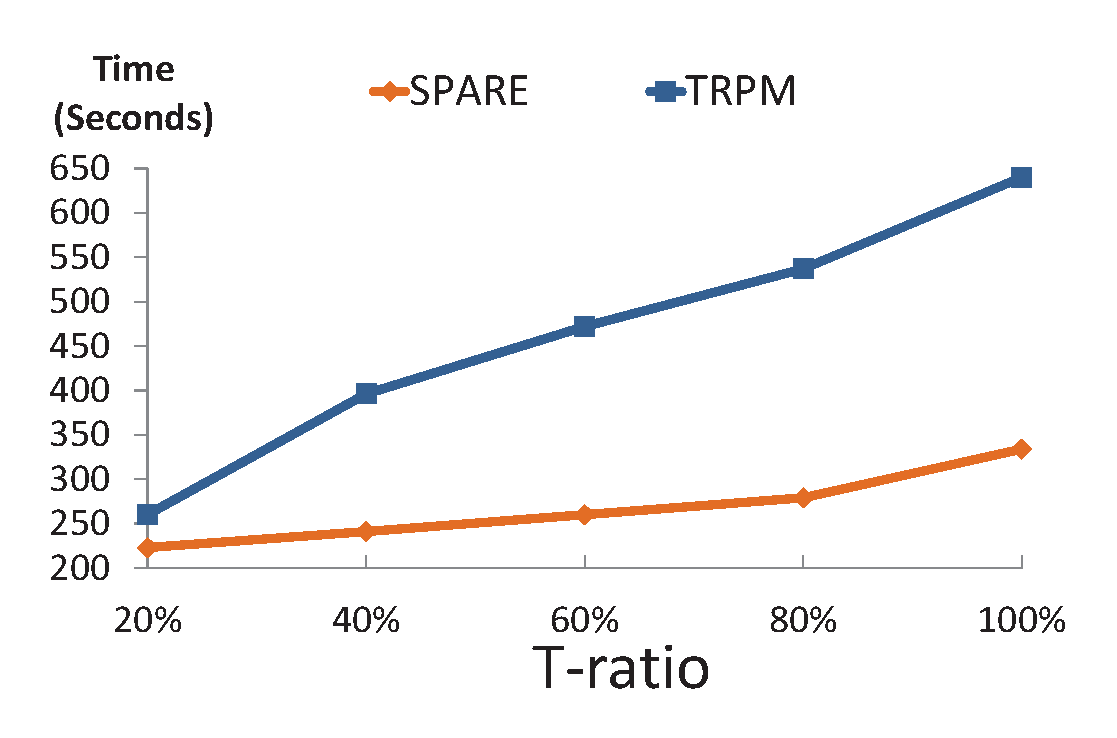
\includegraphics[width=\textwidth]{/exp/performance/shopping_vary_t.eps}
%        \caption{Shopping vary $T_r$}
%    \end{subfigure}
% 	 \begin{subfigure}[b]{0.22\textwidth}
%        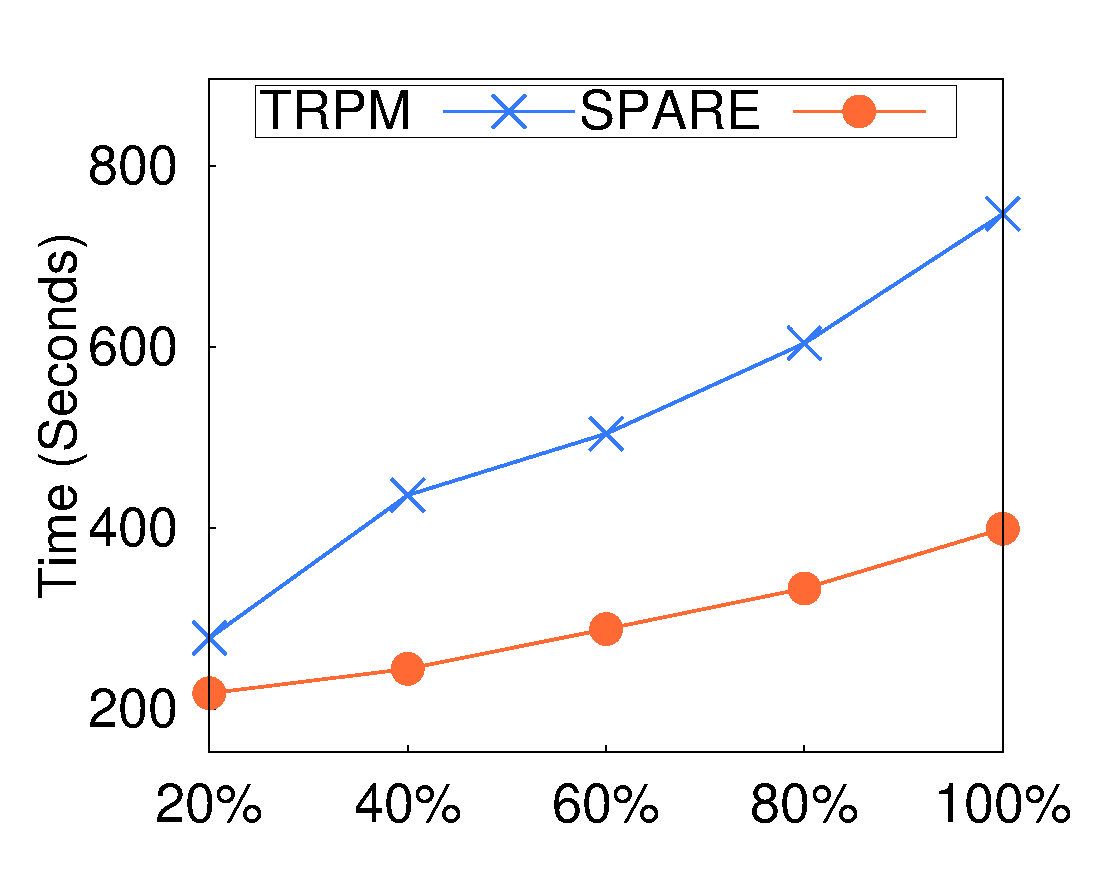
\includegraphics[width=\textwidth]{/exp/performance/geolife_vary_t.eps}
%        \caption{Geolife vary $T_r$}
%    \end{subfigure}
%    	 \begin{subfigure}[b]{0.22\textwidth}
%        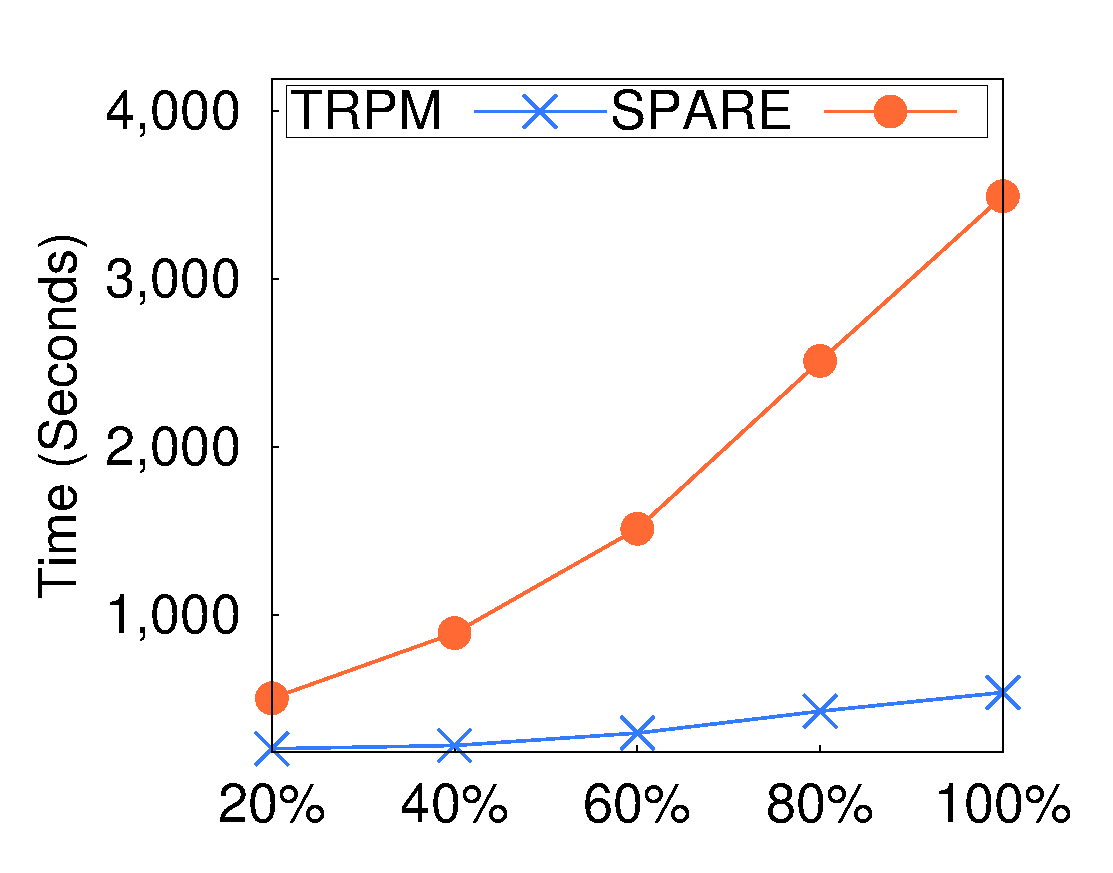
\includegraphics[width=\textwidth]{/exp/performance/taxi_vary_t.eps}
%        \caption{Taxi vary $T_r$}
%    \end{subfigure}
% \caption{Scalability of SPARE and TRPM wrt. $O_r$ and $T_r$}
% \label{exp:performance_vary_OT}
%\end{figure}



\subsection{Analysis of SPARE framework}
In this part, we extensively evaluate SPARE from three aspects:
(1) the advantages brought by the sequence simplification, (2) the effectiveness of load balance, and (3) the scalability with increasing computing resources.
%Then, we study the scalability of SPARE with increasing computing resources.


\subsubsection{Power of sequence simplification}
To study the power of sequence simplification,
we collect two types of statistics: (1) the number of pairs that
are shuffled to the reducers and (2) the number of pairs that
are fed to the Apirori Enumerator. The difference between these two values is the number of size-$2$ candidates pruned by the sequence simplification.
The results in Table~\ref{tbl:pruning} show that the \emph{sequence simplification} is very powerful and eliminates nearly 90 percent of the object pairs, which significantly reduces the overhead of subsequent Apriori enumerator.

\begin{table}[h]
\centering
\begin{tabular}{|l|c|c|c|}
\hline 
\textbf{Dataset} & \textbf{Shopping} & \textbf{GeoLife} & \textbf{Taxi} \\ 
\hline 
Before pruning & 878,309 &  1,134,228 & 2,210,101 \\ 
\hline 
After pruning & 76,672 & 123,410 & 270,921 \\ 
\hline 
Prune ratio & 91.2\% & 89.1\% & 87.7\% \\ 
\hline 
\end{tabular} 

\caption{Pruning power of SPARE.}
\label{tbl:pruning}
\end{table}

\begin{figure}[h]
\centering
	  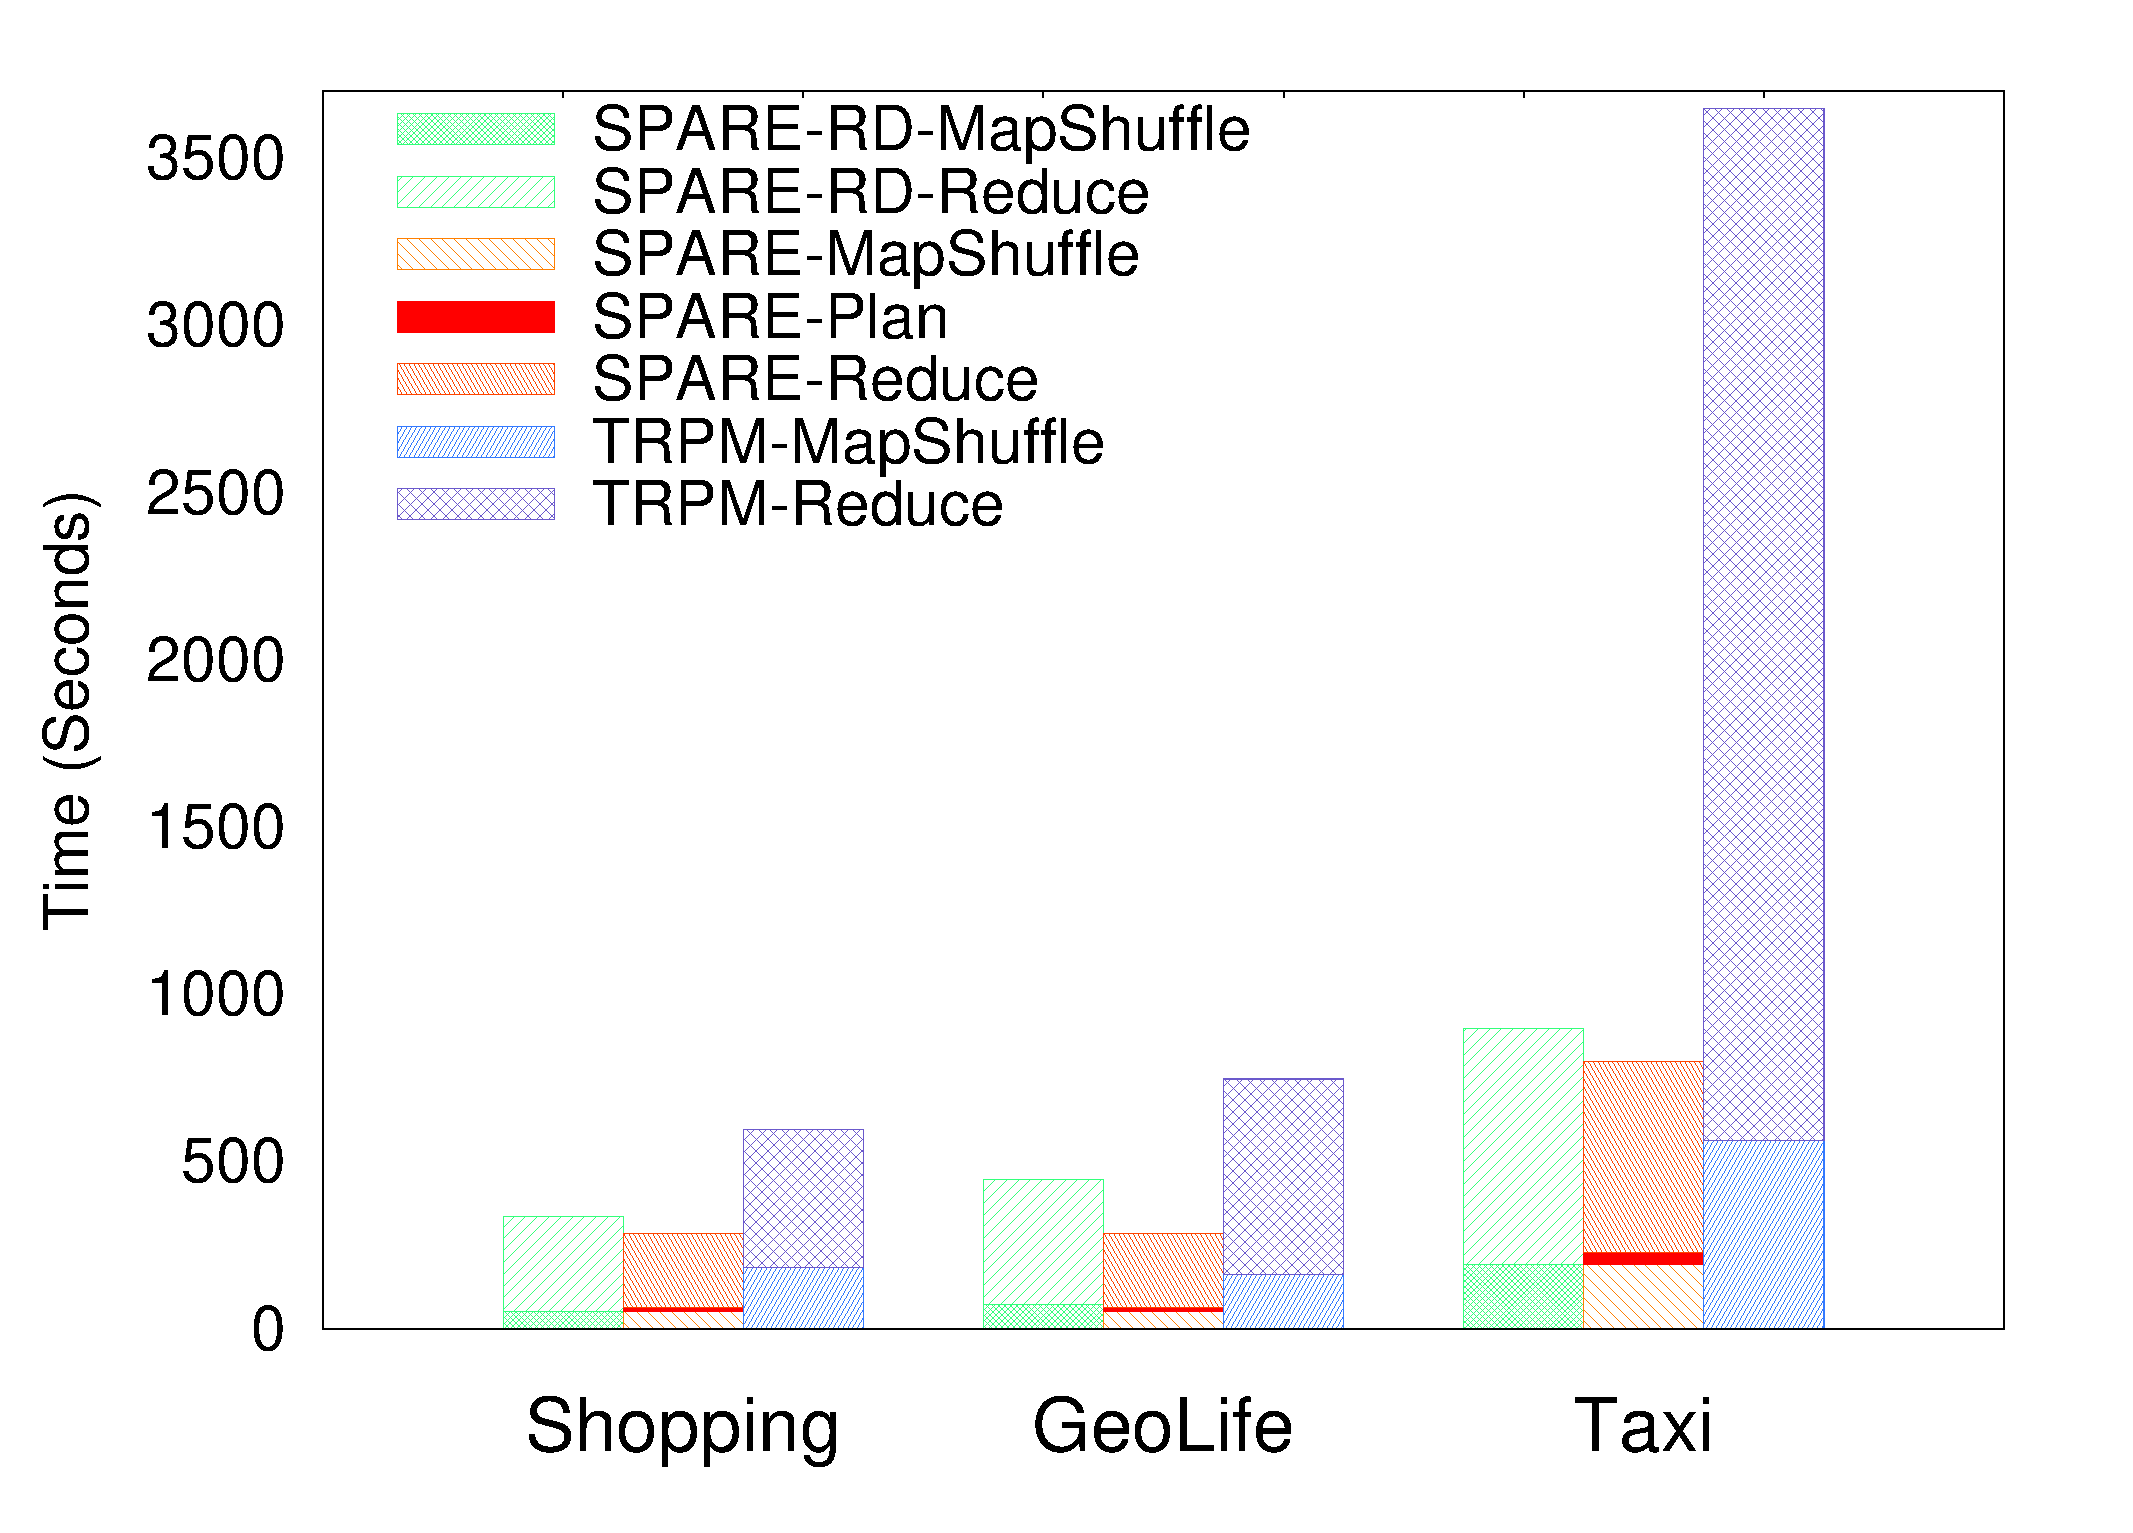
\includegraphics[width=0.35\textwidth]{/exp/spare/detail1.eps}
    \caption{Breakdown of cost of TRPM, SPARE and SPARE-RD.}
    \label{exp:wl}
\end{figure}

\begin{table}[h]
\centering \small
%\begin{tabular}{|c|c|c|c|c|}
%\hline
%\multirow{2}{*}{\textbf{Dataset}} & \multicolumn{2}{c|}{\textbf{SPARE-RD}} & \multicolumn{2}{c|}{\textbf{SPARE}} \\ \cline{2-5} 
%                         & Straggler        & Std. Dev.     & Straggler       & Std. Dev.      \\ \hline
%Shopping                 & 295              & 41         & 237             & 21       \\ \hline
%GeoLife                  & 484              & 108        & 341             & 56       \\ \hline
%Taxi                     & 681              & 147        & 580             & 96       \\ \hline
%\end{tabular}
\begin{tabular}{|l|c|c|c|c|}
\hline
\multicolumn{1}{|c|}{\textbf{Dataset}} & \textbf{Method} & \textbf{Min} & \textbf{Max} & \textbf{Std. Dev.} 
\\ \hline%\specialrule{1pt}{-0.5pt}{-0.5pt} 
\multirow{3}{*}{Shopping}              & TRPM            &     426                          & 597                 & 35 
\\ %\cline{2-5} 
                                       & SPARE-RD          & 122                               &  295             & 41
\\% \cline{2-5}                                        
									   & SPARE           &  134                              &   237               & 21
\\ \hline                                
\multirow{3}{*}{GeoLife}              & TRPM            &    493                            & 747                & 78               \\ %\cline{2-5} 
                                       & SPARE-RD          &  38                               &   484               & 148
\\ %\cline{2-5}                                        
									   & SPARE           &   107                             &     341             & 96
\\ \hline
\multirow{3}{*}{Taxi}              & TRPM            &   3,460                            &    3,648              & 51 \\ %\cline{2-5} 
                                       & SPARE-RD          & 122                               & 681                 & 109
\\ %\cline{2-5}                                        
									   & SPARE           &   134                             &  580                & 56               
\\ \hline
\end{tabular}
  \caption{Statistics of execution time (in seconds) among all executors.}
  \label{tbl:strags}
\end{table}

\subsubsection{Load balance}
To study the effect of load balance in the SPARE framework, we use random task allocation (the default setting of Spark) as a baseline, denoted by SPARE-RD, and compare it with our best-fit method. In best-fit, the largest unassigned star is allocated to the currently most lightly loaded reducer.
Figure~\ref{exp:wl} shows the breakdown of the costs in the map-reduce stages 
for SPARE and SPARE-RD \revised{with TRPM as comparison}. We observe that the map and shuffle time of SPARE and SPARE-RD are identical . The difference is that SPARE incurs an additional overhead to generate an allocation plan for load balance (around $4\%$ of the total cost), resulting in significant savings in the reduce stage (around $20\%$ of the total cost). 
\revised{Meanwhile, both SPARE and SPARE-RD outperform TRPM in each phase. This indicates the 
efficiency of the star partition and apriori enumeration.} 
\revised{We also report the cost summaries (i.e., longest, shortest and standard deviation) of all jobs for the three methods in Table~\ref{tbl:strags}. As the table shows, SPARE produces more balanced jobs
than SPARE-RD which verify the effectiveness of the best-fit strategy. In addition, TRPM 
maintains a low deviation because it uses equal size (i.e., $\eta$) partitioning. 
However, TRPM still takes much longer time than SPARE algorithms.}
%We also report the cost  for all jobs in Table~\ref{tbl:strags}, whose results clearly verify the effectiveness of our allocation strategy for load balance.
%We also report the cost of \emph{straggler}, i.e., the longest job, and the standard deviation (Std. Dev.) for all jobs in Table~\ref{tbl:strags}, whose results clearly verify the effectiveness of our allocation strategy for load balance.

\subsubsection{Scalability}
When examining SPARE with increasing computing resources (number of machines), we also compare SPARE with the state-of-the-art solutions for \emph{swarm} and \emph{platoon} in the single-node setting. Since the original \emph{swarm} and \emph{platoon} detectors cannot handle very large-scale datasets, we only use 60\% of each dataset for evaluation. To make fair comparisons, we customize two variants of SPARE to mine \emph{swarm}s and \emph{platoon}s, which are denoted as SPARE-S and SPARE-P respectively. The customization is according to the settings in Table~\ref{tbl:patterns} and the results are reported in Figure~\ref{exp:scalability}. 
First, the centralized schemes are not suitable to discover patterns in 
large-scale trajectory databases. It takes nearly $30$ hours to 
detect \emph{swarm}s and $11$ hours to detect \emph{platoon}s in the Taxi dataset in a single machine. 
In contrast, when utilizing the multi-core \revised{(i.e., a single node with four executors)} environment, 
SPARE-P achieves $7$ times speedup and SPARE-S achieves $10$ times speedup. 
%our TRPM and SPARE achieves 2.4 times and 7.1 times speedup respectively. 
Second, we see that SPARE schemes demonstrate promising scalability in terms of the number of machines available. The running times decrease almost inversely as more machines are used. 
When all the $11$ nodes ($162$ cores) are available, 
SPARE-P is upto $65$ times and SPARE-S is upto $112$ times better than the state-of-the-art centralized schemes.
%than \emph{platoon} and SPARE-S is upto $112$ times better than \emph{swarm}.
%state-of-the-art \emph{platoon} detector in a centralized server.

\begin{figure*}[t]
\centering
\begin{subfigure}[b]{0.31\textwidth}
    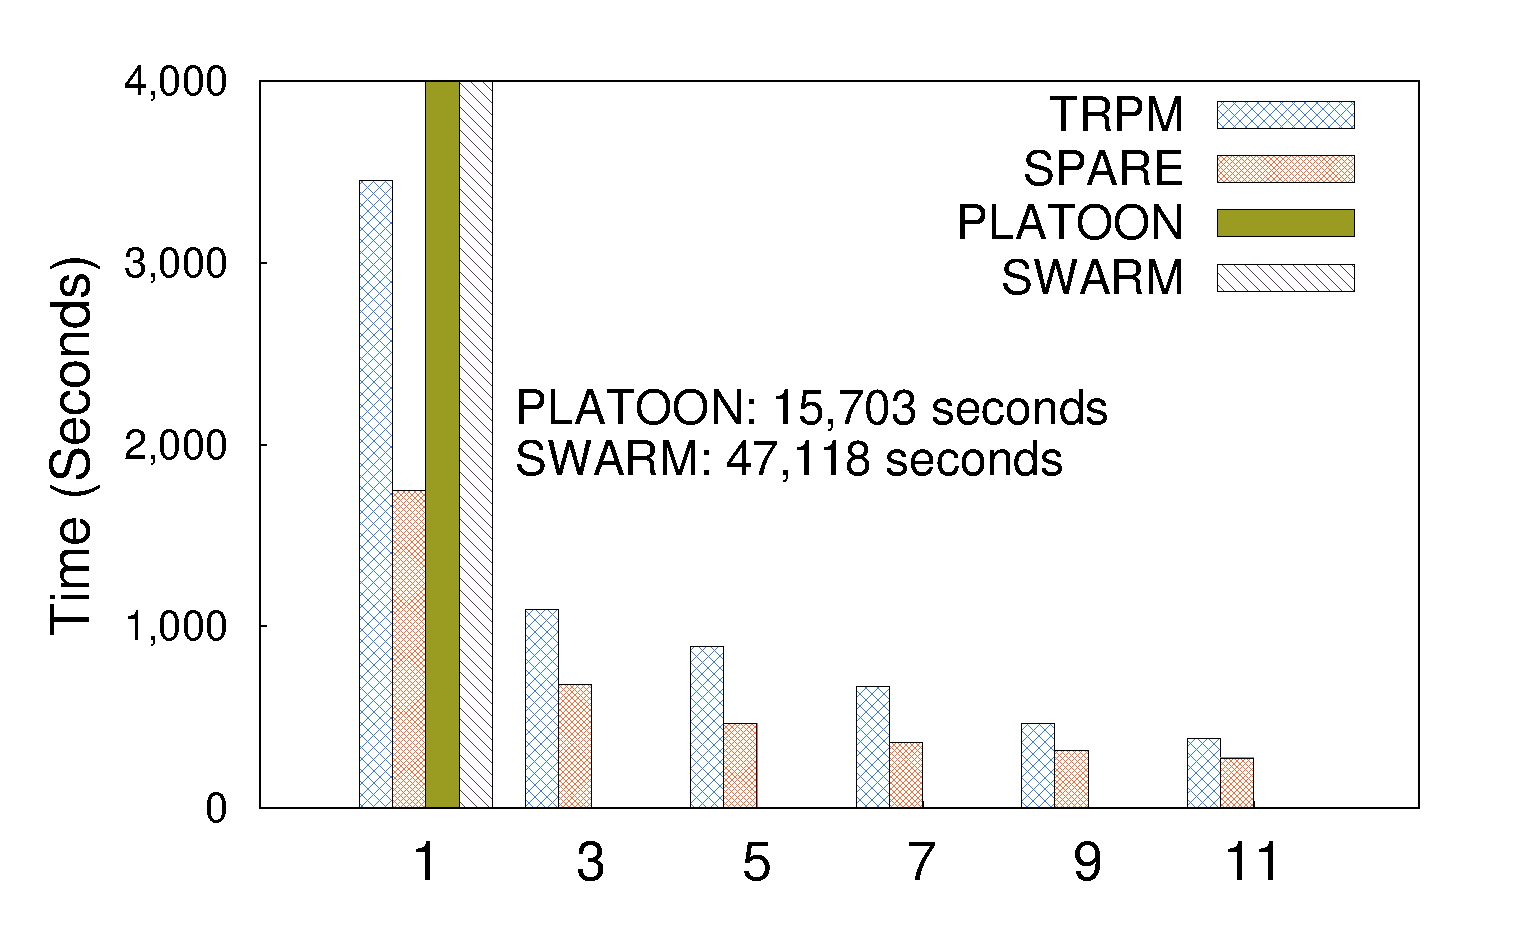
\includegraphics[width=\textwidth]{/exp/spare/scalability-shopping.eps}
        \caption{Shopping vary $N$}
    \end{subfigure}
 	 \begin{subfigure}[b]{0.31\textwidth}
        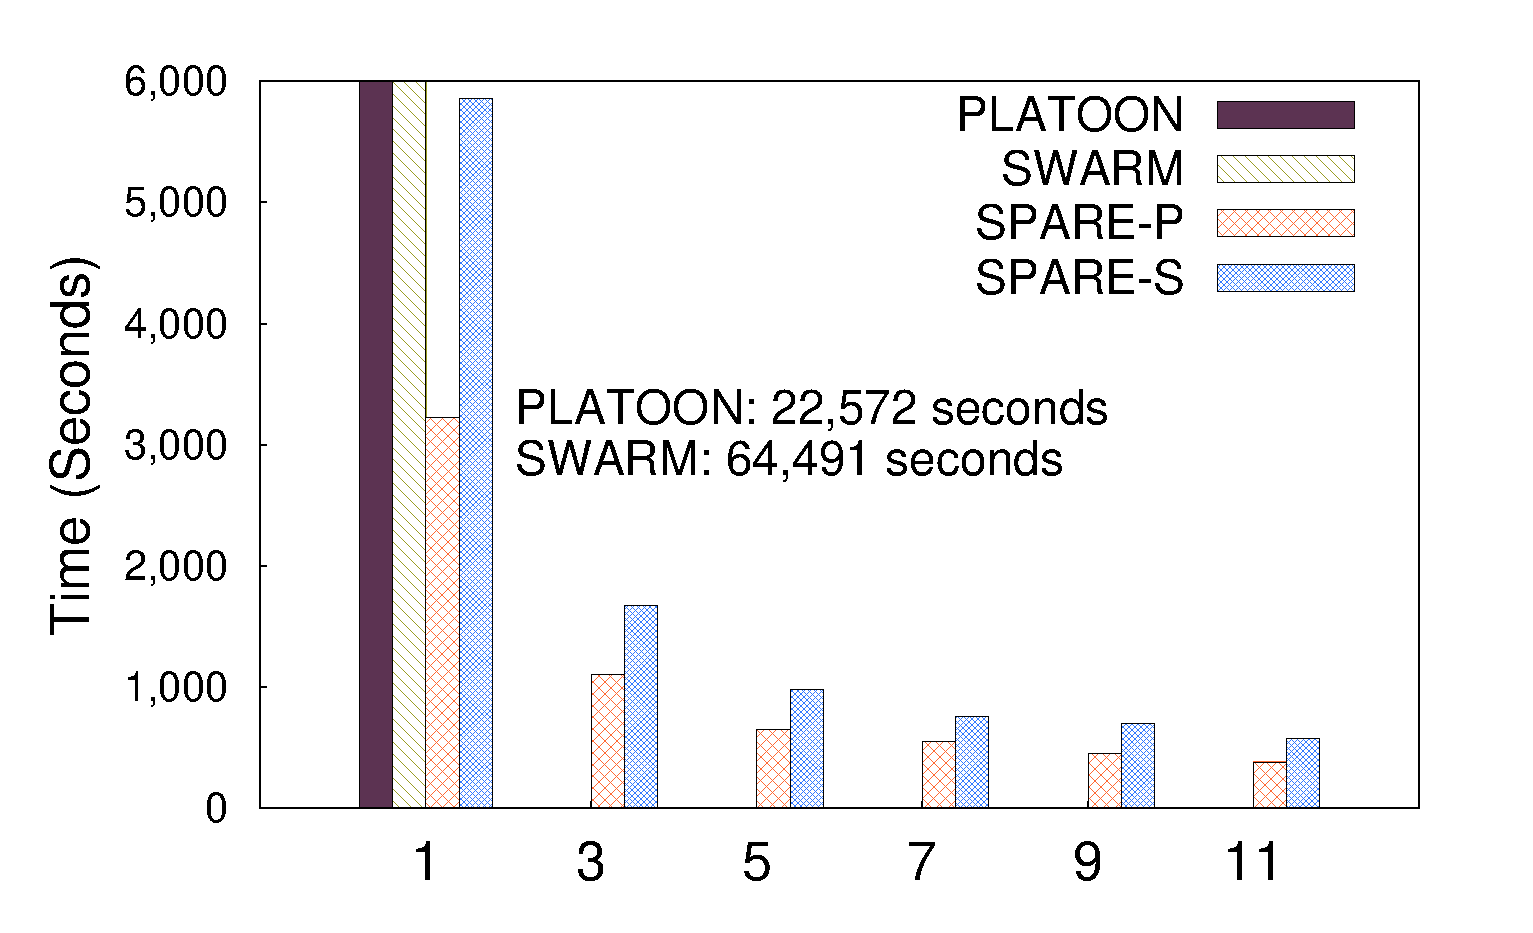
\includegraphics[width=\textwidth]{/exp/spare/scalability-geolife.eps}
        \caption{GeoLife vary $N$}
    \end{subfigure}
    	 \begin{subfigure}[b]{0.31\textwidth}
        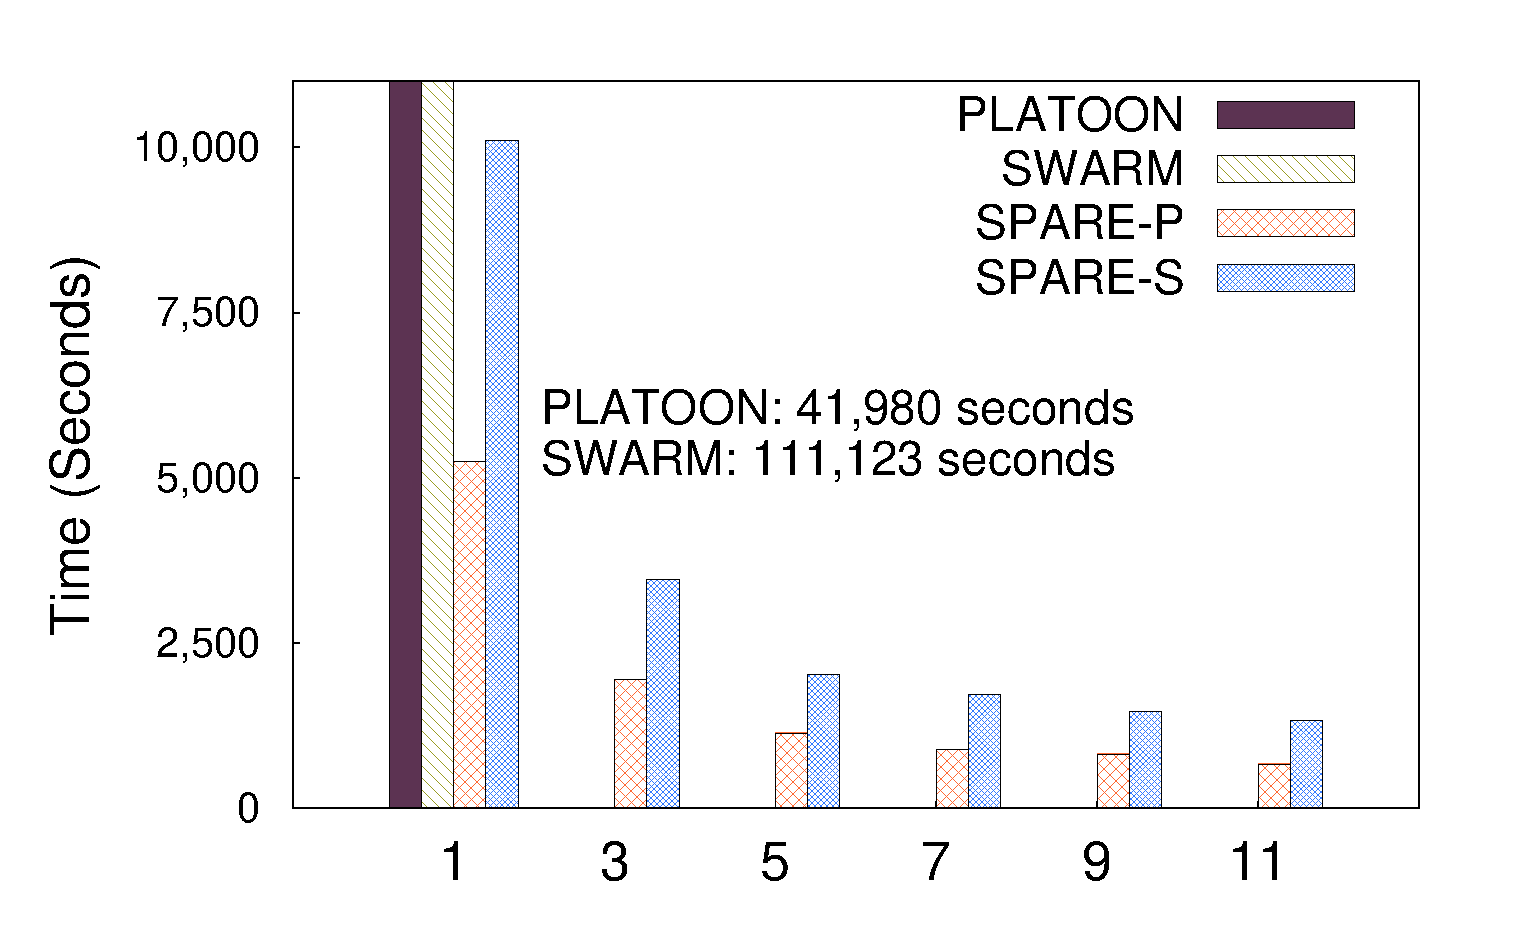
\includegraphics[width=\textwidth]{/exp/spare/scalability-taxi.eps}
        \caption{Taxi vary $N$}
    \end{subfigure}
 \caption{Comparisons among TRMP, SPARE, PLATOON and SWARM.}
 \label{exp:scalability}
\end{figure*}
